
\section{Stochastic differential equations (SDE)}

A proper testbed for EWS is to  simulate what happens in a dynamical system when noise is part of the dynamic and a control parameter changes continuously,  and see if we can predict its transition.

Since real systems (and measurements) have noise, this is particularly relevant in systems where the noise can  affect the dynamics of the system \citep{Coulson2004}.

Such systems meed to  be described by some differential equation that has the noise incorporated in the integration scheme, i.e. stochastic differential equations (SDE). Though technically speaking the differential equation is no longer continuous since there are stochastic perturbations at each integration step, and therefore there is a fractality to the way the noise exists in these equations, there are  many cases in which these equations can be solved in a probabilistic sense. 


This means that each integration now is just a path of the many possible paths the system can take in its evolution, each one with some probability. 


%\subsection{Simulations on stochastic differential equations}

We consider a deterministic nonlinear differential equation $\dot{\vec x}=f(\vec x,\vec \lambda)$, which in this context will be called \textit{deterministic backbone}, where $\vec x$ is a variable of the system and, for our purposes the observable, and $\vec \lambda$ is a set of parameters of the system.

In general, we can consider a system which can not only have some constant internal noise but also be perturbed by 'kicks'.
Such a system can be simulated as a drift-diffusion-jump model: 
\begin{equation}
	\mathop{d\vec x}=f(\vec x,\vec \lambda)\mathop{dt}+g(\vec x,\lambda)\mathop{dW}+c\mathop{dJ}
	\label{eq: SDE general}
\end{equation}

In this case $f(\vec x,\vec \lambda)$ is the deterministic backbone of the equation, $g(\bar x,\bar \lambda)$ is the noise intensity which can include interaction between the data and the noise, $\mathop{dW}$ is a Gaussian (white noise) process (Wiener process) with zero mean and unit variance ($N(0,1$)) and $\mathop{dJ}$ is a Poisson process with positive intensity $c$. 
If the function $g(x,\lambda)=\sigma$, then the system has additive noise; if $g(x,\lambda)=\sigma x$, the process has multiplicative noise.

In equation \eqref{eq: SDE general}, the Wiener process implies a constant white noise, while the Poisson process models occasional perturbations in the system, usually called 'jumps' or 'kicks' \citep{bibid}.

This means that besides the freedom we have when selecting the speed at which the parameter changes ($\la=\la(t)$), we also have freedom on the choice in the noise intensity, and the process from which it comes from, which influences the color of the noise \citep{Kaur2022}. 

Each of this options greatly complexifies our analysis. Even when considering only Wiener processes, there are fundamental differences between additive and multiplicative noise \citep{Alberti2021} since multiplicative noise effectively can change the dimensionality of attractors and  the stable manifolds in a different way from additive noise. 
Even only considering additive noise, having some correlation on the noise can change bifurcation points and early warning performance as shown by \cite{Kaur2022}.


For the sake of simplicity, in this work we will focus on  one dimensional systems with additive white noise. 



\subsection{Ornstein-Uhlenbeck stochastic process}


Our autonomous system now reads\footnote{This can also be written in a Langevin equation of the form 
	\begin{equation}
		\frac{\mathop{dx}}{\mathop{dt}}=  f(x,\lambda)  + \sigma \eta(t)  
		\label{Langev UB process}
	\end{equation}
	where $\eta(t)$ is white noise $N(0,1)$. It is also possible to represent this as a Focker-Planck equation.}
\begin{equation}
	\mathop{dx}=f(x,\lambda) \mathop{dt} + \sigma \mathop{dW}
	\label{eq: pre_U-B process}
\end{equation}
where $ \sigma>0$. 



%This type of process has the properties of being a Gaussian process, a Markov process and temporally homogeneous (similar to a random walk).

%Near the equilibrium of the deterministic backbone $x^*$, this system with additive white noise can be written as a Ornstein-Uhlenbeck stochastic process\citep{bibid}.

In this case, for large enough times (after the transient), if the noise is small enough, and the system relaxes to a stable equilibrium, then it can be approximated as an Ornstein-Uhlenbeck process:
\begin{equation}
	\mathop{dx}=||M||(x-x^*)  \mathop{dt} + \sigma \mathop{dW}
	\label{eq: U-B process}
\end{equation}
 which allows us to estimate the first two moments of the ensemble of paths of  $x(t)$ and the autocorrelation at lag-1. In this case, the mean is equal to the equilibrium of the deterministic backbone $x^*$ (for $\la=$constant):
\begin{equation}
	\lim_{t\to\infty} E[x]=x^*
		\label{eq: mean}
\end{equation}
and the variance ($Var[x]$) for an initial condition in the vicinity of the equilibrium is:
\begin{equation}
	\mathrm{Var}[x]=\frac{\sigma^2}{2 ||M(x^*,\lambda)||}(1-e^{-2Mt}).
	\label{eq: ST_variance}
\end{equation}

This also allow us to define a relaxation time for the noise, which is half the relaxation time of the deterministic backbone ($t_\mathbb{relax}\approx 1/2M$). This also defines the correlation time $t_{\mathrm{corr}}=t^*/2$, and therefore the minimum time interval to use in our analysis windows. 
In this case the variance  relaxes to 
\begin{equation}
	\lim_{t\to\infty} \mathrm{Var}[x]=\frac{\sigma^2}{2f'(x^*,\lambda)}=\frac{\sigma^2}{2 ||M(x^*,\lambda)||}
	\label{eq: ST_variancelim}
\end{equation}
so we can see how the variance diverges when $M$ tends to zero.

In this case we can also calculate the expected autocorrelation. 
If the data points are spread evenly by $\Delta t$, then the lag-1 is \citep{Ritchie2016}:
\begin{equation}
	\mathrm{Lag}_{1}=e^{-M\Delta t }\approx 1-M\Delta t
	\label{eq:lag1}
\end{equation}
this give us a tool to approximate the LDR as
\begin{equation}
	M=-\frac{\mathrm{Lag}_1-1}{\Delta t}
	\label{eq:Mfromlag1}
\end{equation}
or through the variance as 
\begin{equation}
	M=-\frac{\sigma^2}{2 \mathrm{Var}}.
	\label{eq:Mfromvar}
\end{equation}

From the expressions of the equilibrium variance and lag-1 we can see that 
\begin{equation}
	\mathrm{Var}\frac{\mathrm{Lag}_{1}-1}{\, \Delta t}\approx \frac{\sigma^2}{2}=const
	\label{eq:constante}
\end{equation}
which has been proposed as a way to discern between signals of critical transitions and transitions due to other mechanisms \citep{..}.


All these results for the OU process require some de-trending of the data when the control parameter is free to change, since these equations are valid only around the equilibrium (they should be calculated on the residual noise of the detrending).

Choosing a detrending algorithm presents its own set of challenges. 
In our case we follow \citep{..} in the use of moving average with a Gaussian kernel (with  a proper choice of bandwidth). 
Since we want our EWS to be usable on single realizations (since in general we don't have access to several copies of the same system to make an ensemble), recovering these results warrants not only enough data to be able to have reliable statistics (and representative samples), but also windows big enough to span several correlation windows. 
For evenly spaced data and constant window width for the analysis, it is clear that at some point, if the system approaches a critical transition, this requirements will not be satisfied as the correlation time tends diverges at the bifurcation.

We refer to \cite{Ritchie2016} for approximations on the possible escape paths for an R-tipping system with noise.

\subsection{Augmented stochastic  system (ASS)}
Now our full non-autonomous system can be written as an augmented system of eq.\eqref{eq: pre_U-B process}:
\begin{equation}
	\begin{cases}
		d x&=f(x,\lambda)\,dt+\sigma\, dW,\\
		d \la &= c_\lambda\, dt \neq 0.
	\end{cases}
\end{equation}

%\textcolor{red}{For the sde, the correlation time can be estimated as }
%
%\begin{equation}
% 		t_{corr}=\sqrt{t^*}
%\label{eq: corrl_time}
%\end{equation}
%

Numerical integration is done using  the Heun scheme in the module -stratHeun- from the sdeint Python package\footnote{We use Version 0.3.0, the latest at the time of writing. The project can be found at \href{https://pypi.org/project/sdeint/}{https://pypi.org/project/sdeint/} .} which follows the scheme presented by \cite{Mannella2002,Burrage}.



Even only considering additive noise, there are still many possibilities to take into account since we have the freedom of noise intensity and parameter speed. 

To further narrow our scope, we will only work with slow variation of the bifurcation parameter and with small noise, since we need to know if and when we can predict B-tipping in the simplest scenario before moving to more challenging frameworks. 
This means to consider the case of a slow drift of a parameter nearing a bifurcation, where the system still behaves following the dynamics of the manifold  similar to the case of a constant parameter. 

\begin{figure}[htb]
	\centering
	\begin{tikzpicture}
		\draw (0,0) node[rectangle, thin,left color=blue!90, right color=orange!90,shading angle=90,anchor=south west, minimum height=3cm,minimum width=5cm,opacity=0.7] (R1) at (0,0){};
		\draw (0,0) node[rectangle, thin,left color=green!80, right color=red!80,shading angle=180,anchor=south west, minimum height=3cm,minimum width=5cm,opacity=0.4] (R1) at (0,0){};
		\draw [->,opacity=1,very thick](R1.south west) node[below] {} -- (R1.south east)  node[right] {Noise} node[below] {large};
		\draw [->,opacity=1,very thick](R1.south west) node[left] {} -- (R1.north west) node[above] {Parameter speed} node[left] {fast} ;
		%\node (a) at (0.38,0.38) {};
		\draw [dashed,opacity=0.8,thick](R1.south) -- (R1.north) node {} ;
		\draw [dashed,opacity=0.8,thick](R1.west) -- (R1.east)  node {};
		%	\node[circle,draw,minimum size=10cm] (a) at (0,0) {};
		\node (a) at (0.08,0.08) {};
		\draw [dotted,thick] (R1.south west) circle [radius=0.3cm,draw=black] ;
		\filldraw [blue!70!green!80!black!90,thick] (a.center) circle [radius=0.13cm,draw=black];
		\node (e) at ($(R1.south west)!0.5!(R1.center)$) {$1$};
		\node (e) at ($(R1.south east)!0.5!(R1.center)$) {$2$};	
		\node (e) at ($(R1.north west)!0.5!(R1.center)$) {$3$};	
		\node (e) at ($(R1.north east)!0.5!(R1.center)$) {$4$};
		\node (a) at (R1.south) {};
%		\node (b) [below=0.1cm of a]  {$\sigma\sqrt{\frac{1}{2M}}\approx \mathcal{B}$};
		\node (b) [below=0.1cm of a]  {$\mathrm{noise} \approx \mathrm{basin}$};
		\node (a) at (R1.west) {};
%		\node (b) [left=0.1cm of a]  {$\frac{1}{||M||}\int \frac{d\la}{c_{\la}} \approx 1$};
		\node (b) [left=0.1cm of a]  {$t_{\mathrm{sweep}} \approx t^*$};
	\end{tikzpicture}
	\caption{We focus on slow change of parameters and small additive noise\footnote{CSD early warning work better for small noise. As with r-tipping, there will be a definition for the noise related to the tipping and another related to the goodness of the CSD theroy application.}.}        
	\label{fig: noise_transition}
\end{figure}
 
We need to develop a definition to quantify 'small' and 'slow' in this case, when the bifurcation implies a change of sign in the real eigenvalue of the fixed point. 
 
Figure \ref{fig: noise_transition} shows an example of the case we want to study (blue circle). 
In this example a 'slow' or 'adiabatic' augmented stochastic system (ASS\footnote{best acronym ever}) is only well defined in a small area, where noise is small enough for the system to not tip outside the basin far from the bifurcation, but also to be able to approximate the system being close to the equilibrium. On the other hand, we want the parameter to move slowly enough for R-tipping to not be a main mechanism of tipping, and to have the system bifurcate close to the expected parameter \citep{Marconi2020a}.%, but also to consider the noise at an equilibrium state and not have significant delays in tipping 

This defines three main areas:
\begin{enumerate}
	\item Slow parameter and low noise: The system is approximately adiabatic\footnote{In the sense of being able to use the results for $M=cte$.} without actually evolving the system step by step in the control parameter, or without any noise. In this case the main mechanism of tipping is attributed mainly to B-tipping. 
	
	\item Slow parameter and large noise: In this case the system evolves slowly but the noise is comparable or larger than the basin of attraction of $x^*$, so N-tipping is a dominant tipping mechanism and there could be a high presence of intermittency between stable states.
	
	\item Fast parameter and low noise: The system can have R-tipping and as we will see, the variance can be affected by the sweeping parameter, which can lead to delays in warnings. The behavior after the bifurcation can also be drastically different depending on the kind of bifurcation.
	\textcolor{red}{Since fast moving parameters can decrease noise, It is not clear if the high noise and high speed could lead to a different behavior of the system.}

	\item \textcolor{red}{it is not completely clear if there is a fourth case or just three}
\end{enumerate}  

Of course these distinctions are actually a part of a spectrum in the ASS system, since if a basin volume decays to zero at the bifurcation, the noise can always tip the system some time before the bifurcation of the deterministic backbone, no matter how small the noise might be. 
On the other side, a sweeping parameter will always move fast close to the bifurcation point, as the characteristic time of the system becomes infinite at the bifurcation. Thus, at some point, it will become large compared to the timescale of the sweeping and the changing parameter speed will become a relevant timescale of the system.

We can also put this in terms of tracking: if $dx^*/d\la \neq0$ then, close enough to the bifurcation, eq.\eqref{eq:Ashwin_track} cannot hold unless\footnote{From \cref{label} if the basin goes to $0$ as the bifurcation approaches, then $R\rightarrow 0$ since $R\leq \mathcal{B}$, while $d_t x^*/M\rightarrow \infty$.} $R=\infty$. 

In other words, there is no such thing as 'low' noise and 'slow' parameter near enough a critical bifurcation. 
However, we still need some definition of adiabatic, which in turn might help us to define when we are close to a tipping zone. 


                     



%\begin{figure}[htb]
%	\centering
%	\begin{tikzpicture}
%		\draw [->,opacity=1](0,0) -- (3.2,0)  node[right] {Noise};
%		\draw ->,opacity=1](0,0) -- (0,3.2) node[above] {Parameter speed} ;
%		\draw (0,0) node[rectangle, thin,left color=blue!80, right color=red!80,shading angle=130,anchor=south west, minimum height=3cm,minimum width=3cm,opacity=0.6] {} {};
%		\node (a) at (0.3,0.3) {};
%		\draw [dashed,opacity=0.8](1.5,0) -- (1.5,3) node {} ;
%		\draw [dashed,opacity=0.8](0,1.5) -- (3,1.5)  node {};
%		%	\node[circle,draw,minimum size=10cm] (a) at (0,0) {};
%		\filldraw [blue] (a.center) circle [radius=0.1cm,draw=black];
%	\end{tikzpicture}
%	\caption{We focus on slow change of parameters and small additive noise.}        
%	\label{fig: noise_transition}
%\end{figure}








%\begin{center}
%	\begin{tikzpicture}[scale=1.5]
		%		% Draw axes
%		\draw [<->,thick] (-2,2) node (yaxis) [above] {$Noise$}
	%	\draw [<->,thick] (-2,2) node (xaxis) [right] {$\dot\theta$};
		%		% Draw two intersecting lines
		%%		\draw (0,0) coordinate (a_1) -- (2,1.8) coordinate (a_2);
		%%		\draw (0,1.5) coordinate (b_1) -- (2.5,0) coordinate (b_2);
		%		% Calculate the intersection of the lines a_1 -- a_2 and b_1 -- b_2
		%		% and store the coordinate in c.
		%%		\coordinate (c) at (-1,-1)
		%%		\draw[dashed] (yaxis |- c) node[left] {}
		%%		-| (xaxis -| c) node[below] {};
		%%		\coordinate (c) at (intersection of (yaxis) and ());
		%		% Draw lines indicating intersection with y and x axis. Here we use
		%		% the perpendicular coordinate system
		%%		\draw[dashed] (yaxis |- c) node[left] {$y'$}
		%%		-| (xaxis -| c) node[below] {$x'$};
		%		% Draw a dot to indicate intersection point
		%%		\fill[red] (c) circle (2pt);
%	\end{tikzpicture}
%\end{center}


\begin{figure}[htbp]
	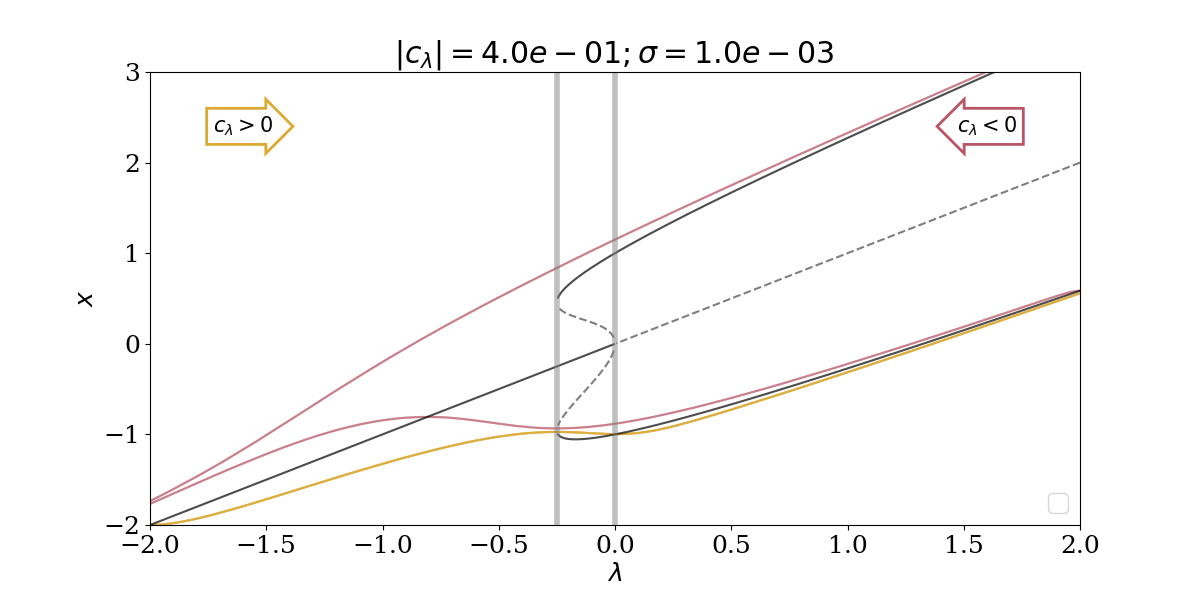
\includegraphics[width=0.49\linewidth]{Images/Metrics/spectrum_cases/slanted_subpitch_fast}
	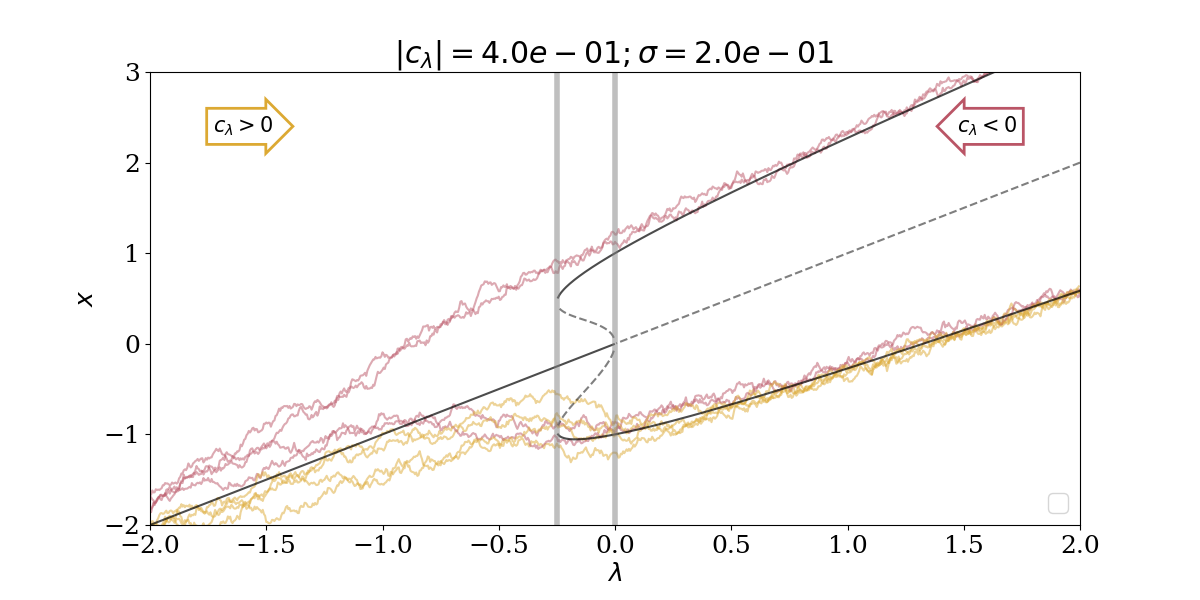
\includegraphics[width=0.49\linewidth]{Images/Metrics/spectrum_cases/slanted_subpitch_fastnoise}\\
	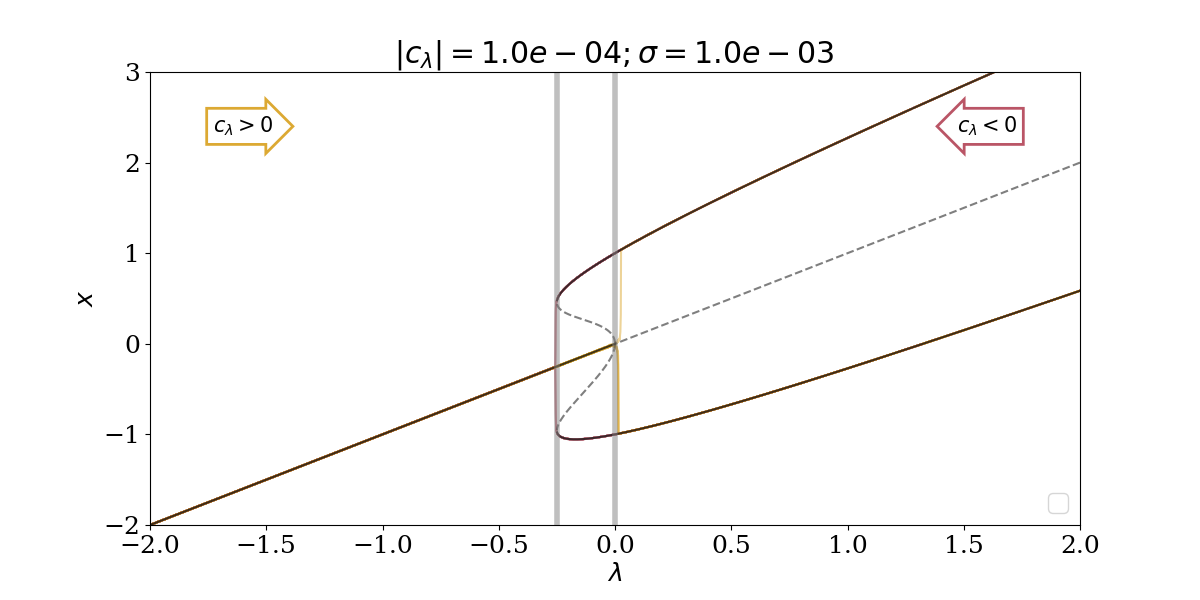
\includegraphics[width=0.49\linewidth]{Images/Metrics/spectrum_cases/slanted_subpitch_adiab}
	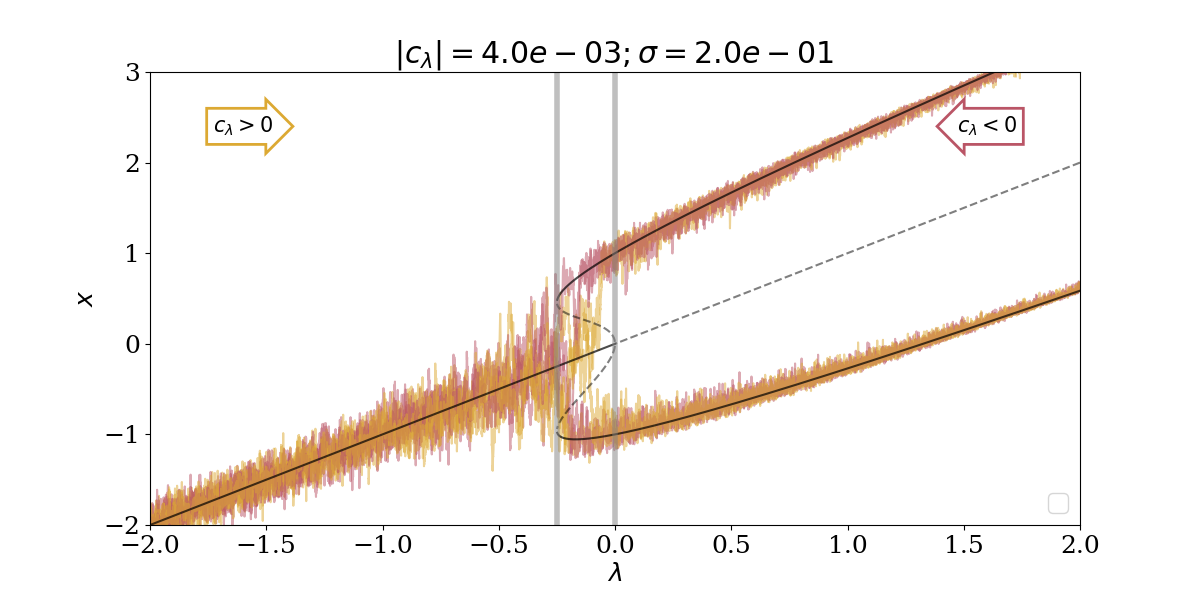
\includegraphics[width=0.49\linewidth]{Images/Metrics/spectrum_cases/slanted_subpitch_noise}
	\caption{Stochastic trayectories of the subcritical pitchfork $dx=\la (x-\la)+(x-\la)^3-(x-\la)^5 dt+\sigma dW$, with fast or slow swiping parameter $\dot{\la}=\left\{0.4,0.004\right\}$ and big or small noise at the bifurcation $\sigma=\left\{0.2,0.01\right\}$. The gray lines mark the bifurcation points for the respective branches.}
	\label{fig: cases}
\end{figure}







